\immediate\write18{tex hobby.dtx}
\documentclass{article}
\usepackage{amsmath}
\usepackage{tikz}
\usetikzlibrary{hobby}

\makeatletter
\tikzset{
  quick curve through/.style={%
    to path={%
      \pgfextra{%
      \tikz@scan@one@point\pgfutil@firstofone(\tikztostart)%
        \edef\hobby@qpointa{\noexpand\pgfqpoint{\the\pgf@x}{\the\pgf@y}}%
        \def\hobby@qpoints{}%
        \def\hobby@quick@path{}%
        \def\hobby@angle{}%
        \def\arg{#1}%
        \tikz@scan@one@point\hobby@quick#1 (\tikztotarget)\relax
      }
      \hobby@quick@path
    }
  }
}

\pgfmathsetmacro\hobby@sf{10cm}

\def\hobby@quick#1{%
  \ifx\hobby@qpoints\pgfutil@empty
  \else
  #1%
  \pgf@xb=\pgf@x
  \pgf@yb=\pgf@y
  \hobby@qpointa
  \pgf@xa=\pgf@x
  \pgf@ya=\pgf@y
  \advance\pgf@xb by -\pgf@xa
  \advance\pgf@yb by -\pgf@ya
  \pgfmathsetmacro\hobby@done{sqrt((\pgf@xb/\hobby@sf)^2 + (\pgf@yb/\hobby@sf)^2)}%
  \pgfmathsetmacro\hobby@omegaone{rad(atan2(\pgf@xb,\pgf@yb))}%
  \hobby@qpoints
  \advance\pgf@xa by -\pgf@x
  \advance\pgf@ya by -\pgf@y
  \pgfmathsetmacro\hobby@dzero{sqrt((\pgf@xa/\hobby@sf)^2 + (\pgf@ya/\hobby@sf)^2)}%
  \pgfmathsetmacro\hobby@omegazero{rad(atan2(\pgf@xa,\pgf@ya))}%
  \pgfmathsetmacro\hobby@psi{\hobby@omegaone - \hobby@omegazero}%
  \pgfmathsetmacro\hobby@psi{\hobby@psi > pi ? \hobby@psi - 2*pi : \hobby@psi}%
  \pgfmathsetmacro\hobby@psi{\hobby@psi < -pi ? \hobby@psi + 2*pi : \hobby@psi}%
  \ifx\hobby@angle\pgfutil@empty
  \pgfmathsetmacro\hobby@thetaone{-\hobby@psi * \hobby@done /(\hobby@done + \hobby@dzero)}%
  \pgfmathsetmacro\hobby@thetazero{-\hobby@psi - \hobby@thetaone}%
  \let\hobby@phione=\hobby@thetazero
  \let\hobby@phitwo=\hobby@thetaone
  \else
  \let\hobby@thetazero=\hobby@angle
  \pgfmathsetmacro\hobby@thetaone{-(2 * \hobby@psi + \hobby@thetazero) * \hobby@done / (2 * \hobby@done + \hobby@dzero)}%
  \pgfmathsetmacro\hobby@phione{-\hobby@psi - \hobby@thetaone}%
  \let\hobby@phitwo=\hobby@thetaone
  \fi
  \let\hobby@angle=\hobby@thetaone
  \pgfmathsetmacro\hobby@alpha{%
    sqrt(2) * (sin(\hobby@thetazero r) - 1/16 * sin(\hobby@phione r)) * (sin(\hobby@phione r) - 1/16 * sin(\hobby@thetazero r)) * (cos(\hobby@thetazero r) - cos(\hobby@phione r))}%
  \pgfmathsetmacro\hobby@rho{%
    (2 + \hobby@alpha)/(1 + (1 - (3 - sqrt(5))/2) * cos(\hobby@thetazero r) +  (3 - sqrt(5))/2 * cos(\hobby@phione r))}%
  \pgfmathsetmacro\hobby@sigma{%
    (2 - \hobby@alpha)/(1 + (1 - (3 - sqrt(5))/2) * cos(\hobby@phione r) +  (3 - sqrt(5))/2 * cos(\hobby@thetazero r))}%
  \hobby@qpoints
  \pgf@xa=\pgf@x
  \pgf@ya=\pgf@y
  \pgfmathsetlength\pgf@xa{%
    \pgf@xa + \hobby@dzero * \hobby@rho * cos((\hobby@thetazero + \hobby@omegazero) r)/3*\hobby@sf}%
  \pgfmathsetlength\pgf@ya{%
    \pgf@ya + \hobby@dzero * \hobby@rho * sin((\hobby@thetazero + \hobby@omegazero) r)/3*\hobby@sf}%
  \hobby@qpointa
  \pgf@xb=\pgf@x
  \pgf@yb=\pgf@y
  \pgfmathsetlength\pgf@xb{%
    \pgf@xb - \hobby@dzero * \hobby@sigma * cos((-\hobby@phione + \hobby@omegazero) r)/3*\hobby@sf}%
  \pgfmathsetlength\pgf@yb{%
    \pgf@yb - \hobby@dzero * \hobby@sigma * sin((-\hobby@phione + \hobby@omegazero) r)/3*\hobby@sf}%
  \hobby@qpointa
  \edef\hobby@quick@path{\hobby@quick@path .. controls (\the\pgf@xa,\the\pgf@ya) and (\the\pgf@xb,\the\pgf@yb) .. (\the\pgf@x,\the\pgf@y) }%
  \fi
  \let\hobby@qpoints=\hobby@qpointa
  #1
  \edef\hobby@qpointa{\noexpand\pgfqpoint{\the\pgf@x}{\the\pgf@y}}%
  \pgfutil@ifnextchar\relax{%
  \pgfmathsetmacro\hobby@alpha{%
    sqrt(2) * (sin(\hobby@thetaone r) - 1/16 * sin(\hobby@phitwo r)) * (sin(\hobby@phitwo r) - 1/16 * sin(\hobby@thetaone r)) * (cos(\hobby@thetaone r) - cos(\hobby@phitwo r))}%
  \pgfmathsetmacro\hobby@rho{%
    (2 + \hobby@alpha)/(1 + (1 - (3 - sqrt(5))/2) * cos(\hobby@thetaone r) +  (3 - sqrt(5))/2 * cos(\hobby@phitwo r))}%
  \pgfmathsetmacro\hobby@sigma{%
    (2 - \hobby@alpha)/(1 + (1 - (3 - sqrt(5))/2) * cos(\hobby@phitwo r) +  (3 - sqrt(5))/2 * cos(\hobby@thetaone r))}%
  \hobby@qpoints
  \pgf@xa=\pgf@x
  \pgf@ya=\pgf@y
  \pgfmathsetlength\pgf@xa{%
    \pgf@xa + \hobby@done * \hobby@rho * cos((\hobby@thetaone + \hobby@omegaone) r)/3*\hobby@sf}%
  \pgfmathsetlength\pgf@ya{%
    \pgf@ya + \hobby@done * \hobby@rho * sin((\hobby@thetaone + \hobby@omegaone) r)/3*\hobby@sf}%
  \hobby@qpointa
  \pgf@xb=\pgf@x
  \pgf@yb=\pgf@y
  \pgfmathsetlength\pgf@xb{%
    \pgf@xb - \hobby@done * \hobby@sigma * cos((-\hobby@phitwo + \hobby@omegaone) r)/3*\hobby@sf}%
  \pgfmathsetlength\pgf@yb{%
    \pgf@yb - \hobby@done * \hobby@sigma * sin((-\hobby@phitwo + \hobby@omegaone) r)/3*\hobby@sf}%
  \hobby@qpointa
  \edef\hobby@quick@path{\hobby@quick@path .. controls (\the\pgf@xa,\the\pgf@ya) and (\the\pgf@xb,\the\pgf@yb) .. (\the\pgf@x,\the\pgf@y) }%
}{\tikz@scan@one@point\hobby@quick}}


\pgfmathparse{rad(atan2(-1,0))}
\show\pgfmathresult
\makeatother

\begin{document}
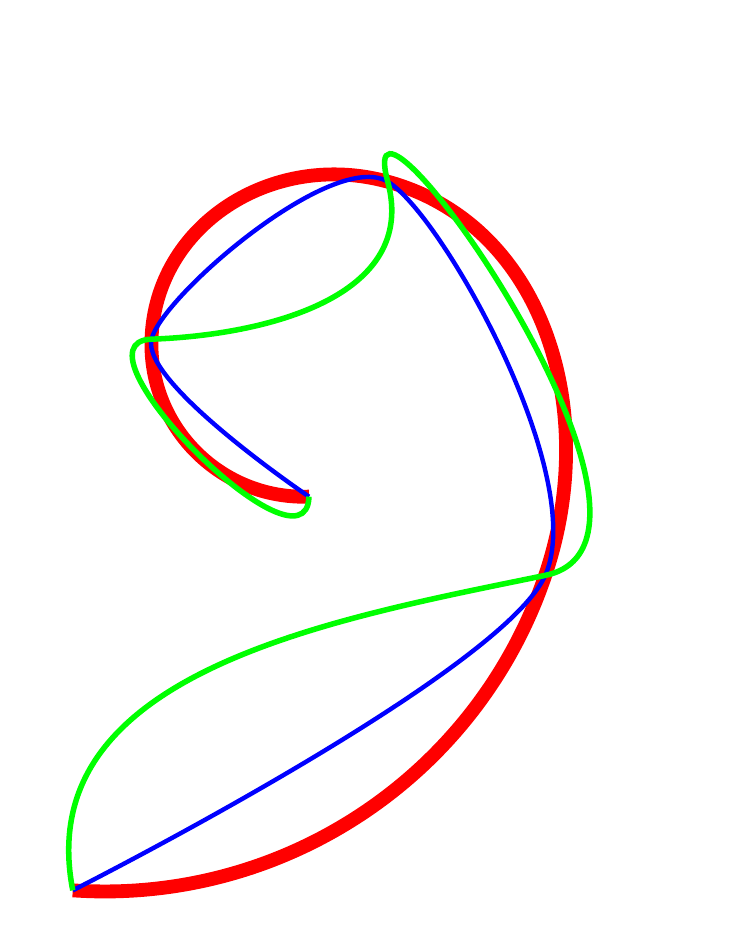
\begin{tikzpicture}
\draw[red,line width=5pt] (0,0) to[curve through={(6,4) .. (4,9) .. (1,7)}] (3,5);
\draw[ultra thick,blue] plot[smooth] coordinates {(0,0) (6,4) (4,9) (1,7) (3,5)};
\draw[green,line width=2pt] (0,0) to[quick curve through={(6,4) (4,9)  (1,7)}] (3,5);
\end{tikzpicture}

\begin{tikzpicture}
\draw[ultra thick,blue] (0,0) .. (1,1) .. (2,0) .. (3,0) .. (2,2) .. (2,4);
\draw[red] (0,0) to[quick curve through={(1,1) (2,0) (3,0) (2,2)}] (2,4);
\end{tikzpicture}

\section{A Piecewise Version of Hobby's Algorithm}

Here we present a variant of Hobby's algorithm.
One difficulty with Hobby's algorithm is that it works with the path as a whole.
It is therefore not possible to build up a path piecewise.
We therefore modify it to correct for this.
Obviously, the resulting path will be less ``ideal'', but will have the property that adding new points will not affect earlier segments.

The method we use is to employ Hobby's algorithm on the two-{}segment subpaths.
This provides two cubic Bezier curves: one from the \(k\)th point to the \(k+1\)st point and the second from the \(k+1\)st to the \(k+2\)nd.
Of this data, we keep the first segment and use that for the path between the \(k\)th and \(k+1\)st points.
We also remember the outgoing angle of the first segment and use that as the incoming angle on the next computation (which will involve the \(k+1\)st, \(k+2\)nd, and \(k+3\)rd) points.

The two ends are slightly different to the middle segments.
On the first segment, we might have no incoming angle.
On the last segment, we render both pieces.

This means that for the initial segment, we have a \(2 \times 2\) linear system:
%
\[
  \begin{bmatrix}
  B_0 & C_0 \\
  A_1 & B_1
  \end{bmatrix}
  \Theta = \begin{bmatrix}
  D_0 \\ D_1
  \end{bmatrix}
\]
%
This has solution:
%
\[
  \Theta = \frac{1}{B_0 B_1 - C_0 A_1} \begin{bmatrix} B_1 & - C_0 \\ -A_1 & B_0 \end{bmatrix} \begin{bmatrix} D_0 \\ D_1 \end{bmatrix} =  \frac{1}{B_0 B_1 - C_0 A_1} \begin{bmatrix} B_1 D_0 - C_0 D_1 \\ B_0 D_1 - A_1 D_0 \end{bmatrix}
\]

Now we have the following values for the constants:
%
\begin{align*}
A_1 &= d_1 \overline{\tau}_2 \overline{\tau}_1^2 \\
%
B_0 &= \tau_0^3 (3 \overline{\tau}_1 - 1) + \chi_0 \overline{\tau}_1^3 \\
%
B_1 &= d_1 \overline{\tau}_2 \overline{\tau}_1^2 (3 \tau_0 - 1) + d_0 \tau_0 \tau_1^2(3 \overline{\tau}_2 - 1) - d_0 \tau_0 \tau_1^2 \frac{\overline{\tau}_2^3 + \chi_2 \tau_1^3 (3 \overline{\tau}_2 - 1)}{\overline{\tau}_2^3 (3 \tau_1 - 1) + \chi_2 \tau_1^3} \\
%
C_0 &= \tau_0^3 + \chi_0 \overline{\tau}_1^3 (3 \tau_0 - 1) \\
%
D_0 &= - (\tau_0^3 + \chi_0 \overline{\tau}_1^3 ( 3 \tau_0 - 1)) \psi_1 \\
%
D_1 &= - d_1 \overline{\tau}_2 \overline{\tau}_1^2 (3 \tau_0 - 1) \psi_1
\end{align*}
%

Let us, for simplicity at the start, assume that the tensions and curls are all \(1\).
Then we have \(A_1 = d_1\), \(B_0 = 3\), \(B_1 = 2 d_1 + 2 d_0 - d_0 = 2 d_1 + d_0\), \(C_0 = 3\), \(D_0 = - 3 \psi_1\), \(D_1 = - 2 d_1 \psi_1\).
Thus the linear system is:
%
\[
  \begin{bmatrix}
  3 & 3 \\
  d_1 & 2 d_1 + d_0
  \end{bmatrix}
  \Theta = - \psi_1 \begin{bmatrix}
  3 \\ 2 d_1
  \end{bmatrix}
\]
%
which we can row reduce to:
%
\[
  \begin{bmatrix}
  1 & 1 \\
  0 & d_1 + d_0 
  \end{bmatrix}
  \Theta = -\psi_1 \begin{bmatrix}
  1 \\ d_1
  \end{bmatrix}
\]
%
whence \(\theta_1 = -\psi_1 \frac{d_1}{d_0 + d_1}\) and \(\theta_0 = -\psi_1 - \theta_1 = -\psi_1\frac{d_0 }{d_0 + d_1}\).
We also compute \(\phi_1 = -\psi_1 - \theta_1 = \theta_0\) and \(\phi_2 = \theta_1\) (in the simple version).
We use \(\theta_0\) and \(\phi_1\) to compute the bezier curve of the first segment, make a note of \(\theta_1\), and -- assuming there are more segments -- throw away \(\phi_2\).

For the inner segments, we have the system:
%
\[
  \begin{bmatrix}
  1 & 0 \\
  A_1 & B_1
  \end{bmatrix}
  \Theta = \begin{bmatrix}
  \theta_0 \\
  D_1
  \end{bmatrix}
\]
%
which has the solution \(\theta_1 = (D_1 - A_1 \theta_0)/B_1\).
The values of the constants in this case are:
%
\begin{align*}
A_1 &= d_1 \overline{\tau}_2 \overline{\tau}_1^2 \\
%
B_1 &= d_1 \overline{\tau}_2 \overline{\tau}_1^2 (3 \tau_0 - 1) + d_0 \tau_0 \tau_1^2(3 \overline{\tau}_2 - 1) - d_0 \tau_0 \tau_1^2 \frac{\overline{\tau}_2^3 + \chi_2 \tau_1^3 (3 \overline{\tau}_2 - 1)}{\overline{\tau}_2^3 (3 \tau_1 - 1) + \chi_2 \tau_1^3} \\
%
D_1 &= - d_1 \overline{\tau}_2 \overline{\tau}_1^2 (3 \tau_0 - 1) \psi_1
\end{align*}

Again, let us consider the simpler case.
Then \(A_1 = d_1\), \(B_1 = 2 d_1 + d_0\), and \(D_1 = - 2 d_1 \psi_1\).
Thus \(\theta_1 = (-2 d_1 \psi_1 - d_1 \theta_0)/(2 d_1 + d_0) = - (2 \psi_1 + \theta_0) \frac{d_1}{2 d_1 + d_0}\).
We compute \(\phi_1 = -\psi_1 - \theta_1 = \frac{- \psi_1 d_0 + \theta_0 d_1}{2 d_1 + d_0}\) and \(\phi_2 = \theta_1\).

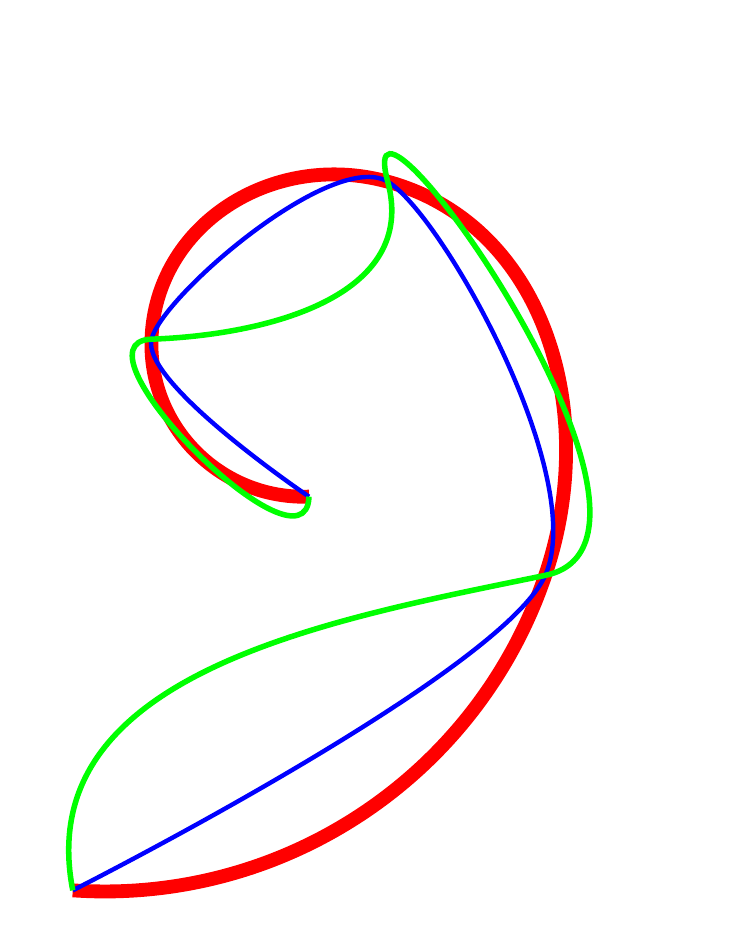
\begin{tikzpicture}
\draw[red,line width=5pt] (0,0) to[curve through={(6,4) .. (4,9) .. (1,7)}] (3,5);
\draw[ultra thick,blue] plot[smooth] coordinates {(0,0) (6,4) (4,9) (1,7) (3,5)};
\draw[green,line width=2pt] (0,0) to[quick curve through={(6,4) (4,9)  (1,7)}] (3,5);
\end{tikzpicture}

\end{document}

\begin{tikzpicture}[c/.style={insert path={circle[radius=2pt]}}]
\fill[green] (0,0) [c] (1,.5) [c] (0,0) [c] (3,.5) [c] (4,0) [c];
\draw (0,0) .. (1,.5) .. (-0.2,0) .. (3,.5) .. (4,0);
\end{tikzpicture}

\begin{tikzpicture}
\draw (0.0000, 0.0000) .. controls (-1.85420, 0.83131) and (1.44747, 2.48215)..(1.0000, 0.5000) .. controls (0.90917, 0.09765) and (0.31923, 0.27721)..(0.1000, 0.0000) .. controls (-1.10155, -1.51937) and (1.46789, -0.02595)..(3.0000, 0.5000) .. controls (3.41450, 0.64229) and (3.86513, 0.41698)..(4.0000, 0.0000);
\end{tikzpicture}

\begin{tikzpicture}
\draw (0.0000, 0.0000) .. controls (0.30056, -0.75821) and (1.42623, -0.19537)..(1.0000, 0.5000) .. controls (0.69595, 0.99605) and (-0.14029, 0.67496)..(0.0000, 0.0000) .. controls (0.31344, -1.50803) and (1.85232, 0.35331)..(3.0000, 0.5000) .. controls (3.40390, 0.55162) and (3.79896, 0.35409)..(4.0000, 0.0000);
\end{tikzpicture}

\begin{tikzpicture}
\draw (0,0) to[curve through={(6,4) .. (4,9) .. (1,7)}] (3,5);
\end{tikzpicture}

\begin{tikzpicture}
\draw (0,0) to[closed,curve through={(6,4) .. (4,9) .. (1,7)}] (3,5);
\end{tikzpicture}
\end{document}


% Local Variables:
% tex-output-type: "pdf18"
% End: